% Chapter Template

\chapter{Results for 2-D Studies} % Main chapter title

\label{Chapter6} % Change X to a consecutive number; for referencing this chapter elsewhere, use \ref{ChapterX}

\lhead{Chapter 6. \emph{Results for 2-D Studies}} % Change X to a consecutive 
%number; this is for the header on each page - perhaps a shortened title

The goal for this section was to see how applicable the method of snapshots and 
the KLT was to 2-D problems.  The C5G7 benchmark was adapted to use a 44-group 
cross-section library, which greatly increased the size of the problem, and 
thus the computation time.  Only the 44-group library was used to generate 
results due to the long computation times necessary to solve for each case.  

Further, in the interest of time, the results for this section have been 
truncated to 10th order.  The overarching goal of the work was to achieve 
sub-$0.1\%$ relative pin 
power errors while reducing the necessary energy degrees of freedom by an order 
of magnitude.  As such, 10th order is sufficient to determine if KLT can reach 
the goal in a 2-D problem-space.

As mentioned previously, the response matrix solution in all 2-D calculations 
was only taken to second order in each angle as well as space, which means that 
the pin powers and fission densities solved by SERMENT will differ 
greatly from the original C5G7 results.  However, the reference case and the 
snapshot models utilized the same spatial and angular order, thus the error 
observed (with respect to the SERMENT reference) is assumed only to be a 
function of the energy expansion order.

\section{Energy Spectra for the Test Problem}

Each of the snapshot models and the full 44-group benchmark problem were solved 
first to provide the spatially averaged flux profiles, which were used for the 
mDLP results.  This spatially averaged spectrum is presented in 
\FIG{fig:c5g7_spectra}.  As compared to the 1-D test problems, the spatially 
averaged spectra are quite distinct between the various models for the 2-D 
problem.  As such, it is expected that mDLP will not perform as well, and 
additionally that effective basis functions will be difficult to attain.

\begin{figure*}[tb]
    \centering
    \includegraphics[trim=.1cm .25cm 2.0cm .4cm clip=true, 
    totalheight=0.28\textheight]{Figures/c/c5g7/rf_plots/%
        44group_spectra_energy}
    \caption{Flux spectrum for the C5G7 problem using 44-group cross-section 
        library}
    \label{fig:c5g7_spectra}
\end{figure*}

\section{Nodal Fission Density Results}

In order to determine the effective constituents for basis function 
construction, several versions of basis functions are derived and compared as 
was done for the 1-D cases.  In this section, each of the results will 
compare the maximum relative error of the nodal fission density for a snapshot 
model.  The nodal fission density is almost equivalent to the assembly power, 
and the reference is taken to the be nodal fission density from a full 
multigroup solution of the C5G7 problem using the 44-group cross-section 
library. First, the results of utilizing snapshots of only the scalar flux 
$\phi$ to generate the KLT basis functions are presented in 
\FIG{fig:c5g7-flux-only}.  In this figure, the maximum relative error of the 
nodal fission density is shown as a function of energy degree of freedom.  

By nine degrees of freedom, none of the models have consistently reached the goal of 
sub-$0.1\%$ errors; however, several models perform well comparatively.  The 
Small-Core model performs well despite spatially reducing the problem by a factor 
of four.  Surprisingly, one of the best performing models is the Combined-Pins model despite the 
simplicity of the model. Both of these snapshot models outperform mDLP and can 
reach nodal fission errors of sub-$1\%$ by at least 7th order.  It would be interesting to view the 
relative performance of the snapshot models are higher-order, but cannot be provided here due to 
time constraints.

As \FIG{fig:c5g7-flux-only} shows, the results of the Small-Core and 
Reduced Small-Core are quite similar, with the Small-Core results being 
slightly better in terms of the maximum relative error.  Due to this 
comparison, it may be assumed that the Reduced Full-Core results are 
approximately equal to the Full-Core results, and thus may be used as a 
comparison point to the best that a basis set can expand the C5G7 solution.

\begin{figure*}[tb]
    \centering
    \includegraphics[trim=.1cm .25cm 2.0cm .4cm clip=true, 
    totalheight=0.28\textheight]{Figures/c/c5g7/rf_plots/phi/%
        energy_basis_comparison_fission-10}
    \caption{Relative error in fission density for 44-group, C5G7 test problem 
using snapshot of only $\phi$.}
    \label{fig:c5g7-flux-only}
\end{figure*}

When the snapshots of only the upward and downward partial current are used for 
basis generation, the results are shown in \FIG{fig:c5g7-current}. Many of the 
cases have improved as compared to using snapshots of only $\phi$ including 
Combined-Pins and Reduced Small-Core.  However, some models have reduced 
effectiveness including Combined-Assemblies and Reduced Full-Core. Unlike the 
1-D case, the partial current 
cannot be assumed symmetric in all directions, thus the partial current in the 
up and down 
directions were chosen.  The combination of up and down was equivalent due to 
symmetry to 
the combination of left and right, thus the choice was made arbitrarily.  

\begin{figure*}[tb]
    \centering
    \includegraphics[trim=.1cm .25cm 2.0cm .4cm clip=true, 
    totalheight=0.28\textheight]{Figures/s/c5g7/rf_plots/partial/%
        partial_energy_basis_comparison_fission-10}
    \caption{Relative error in fission density for 44-group, C5G7 test problem 
        using snapshot of $J_{\text{up}}$ and $J_{\text{down}}$.}
    \label{fig:c5g7-current}
\end{figure*}

\FIGURE{fig:c5g7-combined} presents the results from using snapshots from 
$\phi$, $J_{\text{up}}$, and $J_{\text{down}}$.  The inclusion of the 
partial current had varying effects of the success of each snapshot model, e.g., the reduced 
small-core model was improved in general, while the small-assemblies was worsened.  The 
Combined-Pins results were relatively unchanged, and performed surprisingly well despite the model 
simplicity. The best performing basis sets in general are those that include 
the information of the partial current combined together with the scalar flux.

\begin{figure*}[tb]
    \centering
    \includegraphics[trim=.1cm .25cm 2.0cm .4cm clip=true, 
    totalheight=0.28\textheight]{Figures/c/c5g7/rf_plots/partial/%
        partial_energy_basis_comparison_fission-10}
    \caption{Relative error in fission density for 44-group, C5G7 test problem 
        using snapshot of $\phi$, $J_{\text{up}}$, and $J_{\text{down}}$.}
    \label{fig:c5g7-combined}
\end{figure*}

\section{Pin Power Results}

For an additional comparison for the C5G7 problem, the maximum relative error 
in the pin powers is compared for each of the snapshot models.  The reference 
case for this section is taken as the pin powers from a full multigroup 
solution of the C5G7 problem using the 44-group cross-section 
library.  It is expected that the results in this 
section to be inferior to those in the previous 
section.  Resolving the pin powers is more difficult 
than resolving the nodal fission density, thus more energy degrees of freedom 
should be required to achieve the same level of accuracy. 

\FIGURE{fig:c5g7-flux-only-pp} shows the results utilizing snapshots of only the 
scalar flux $\phi$.  As expected, the results are approximately an order of 
magnitude worse than the equivalent results solving for the fission density.  
However, the same snapshot models all appear to perform the same relative to 
each other.  The best performing case is the Reduced Small-Core, while the 1-D 
Approximation also performs well.  Also note that the Reduced Small-Core 
results are nearly identical to the Small-Core results, which suggests that the 
Reduced Full-Core results may be nearly equivalent to the Full-Core results.  
However, more energy degrees of freedom are needed to resolve the pin powers to 
the desired accuracy.

\begin{figure*}[tb]
    \centering
    \includegraphics[trim=.1cm .25cm 2.0cm .4cm clip=true, 
    totalheight=0.28\textheight]{Figures/c/c5g7/rf_plots/phi/%
        energy_basis_comparison_pinpower-10}
    \caption{Relative error in pin power for 44-group, C5G7 test problem 
using snapshot of only $\phi$.}
    \label{fig:c5g7-flux-only-pp}
\end{figure*}

The performance is somewhat improved when considering only snapshots of the 
partial current in basis generation as shown in \FIG{fig:c5g7-partial-pp}.  For 
this figure, the Small-Core results cannot be shown because too many snapshots 
are available and cannot all be used without running into memory issues.  The 
Reduced Small-Core results must be used as a supplement for the Small-Core 
results.  The Combined-Pins and Reduced Small-Core models perform quite well 
compared to the other snapshot models.

\begin{figure*}[tb]
    \centering
    \includegraphics[trim=.1cm .25cm 2.0cm .4cm clip=true, 
    totalheight=0.28\textheight]{Figures/s/c5g7/rf_plots/partial/%
        partial_energy_basis_comparison_pinpower-10}
    \caption{Relative error in pin power for 44-group, C5G7 test problem 
using snapshot of both $J_{\text{up}}$ and $J_{\text{down}}$.}
    \label{fig:c5g7-partial-pp}
\end{figure*}

When combining snapshots of $\phi$, $J_{\text{up}}$, and $J_{\text{down}}$, the relative 
error in pin power resolution is slightly improved as \FIG{fig:c5g7-combined-pp} shows.  The 
Small-Core model reaches sub-$1\%$ relative 
error by approximately 7th order, provided that the error does not increase 
past the orders shown in the figure.  When using all available snapshots, most 
cases perform better than using only one type of snapshot alone.

\begin{figure*}[tb]
    \centering
    \includegraphics[trim=.1cm .25cm 2.0cm .4cm clip=true, 
    totalheight=0.28\textheight]{Figures/c/c5g7/rf_plots/partial/%
        partial_energy_basis_comparison_pinpower-10}
    \caption{Relative error in pin power for 44-group, C5G7 test problem 
using snapshot of both $\phi$, $J_{\text{up}}$, and $J_{\text{down}}$.}
    \label{fig:c5g7-combined-pp}
\end{figure*}

In order to provide some context for the C5G7 pin power results, a pin power 
heat map for the test problem was created for each of the reference cases.  The 
heat map was designed to view the location of the maximum errors in the test 
problem and related cases. The first heat map is presented in 
\FIG{fig:pin_detran}.  As expected the greatest pin powers are present in the 
UO$_2$ assembly at the center of the model.
    
\begin{figure*}[tb]
    \centering
    \includegraphics[trim=.1cm .25cm 2.0cm .4cm clip=true, 
    totalheight=0.4\textheight]{Figures/c/c5g7/rf_plots/%
        c5g7_ref_detran}
    \caption{Pin power heat map for the DETRAN reference solution.  The 
upper left corner is the center of the core}
    \label{fig:pin_detran}
\end{figure*}

The error of the SERMENT reference solution to the DETRAN solution 
is shown in \FIG{fig:detser}.  In this figure, the center of the model is the 
upper left corner, and the moderator sections of the model have been omitted.  
The greatest error for the SERMENT reference solution occurs at the 
bottom right corner of the figure, which represents a UO$_2$ pin adjacent to 
the moderator section.

\begin{figure*}[tb]
    \centering
    \includegraphics[trim=.1cm .25cm 2.0cm .4cm clip=true, 
    totalheight=0.4\textheight]{Figures/c/c5g7/rf_plots/%
        detser_error}
    \caption{Error of pin powers in the SERMENT reference solution 
relative to the DETRAN reference solution.  The 
upper left corner is the center of the core}
    \label{fig:detser}
\end{figure*}

The error in the pin powers of the best performing KLT case (9th order 
Reduced Small-Core) using only $\phi$ snapshots relative to the SERMENT 
reference solution is presented as a heat map in \FIG{fig:serklt}.  In this 
figure, the maximum error is shown at the center of the figure, which 
corresponds to the center of the reactor quadrant.  The KLT solution also has a 
relatively large error at the assembly boundaries.

\begin{figure*}[tb]
    \centering
    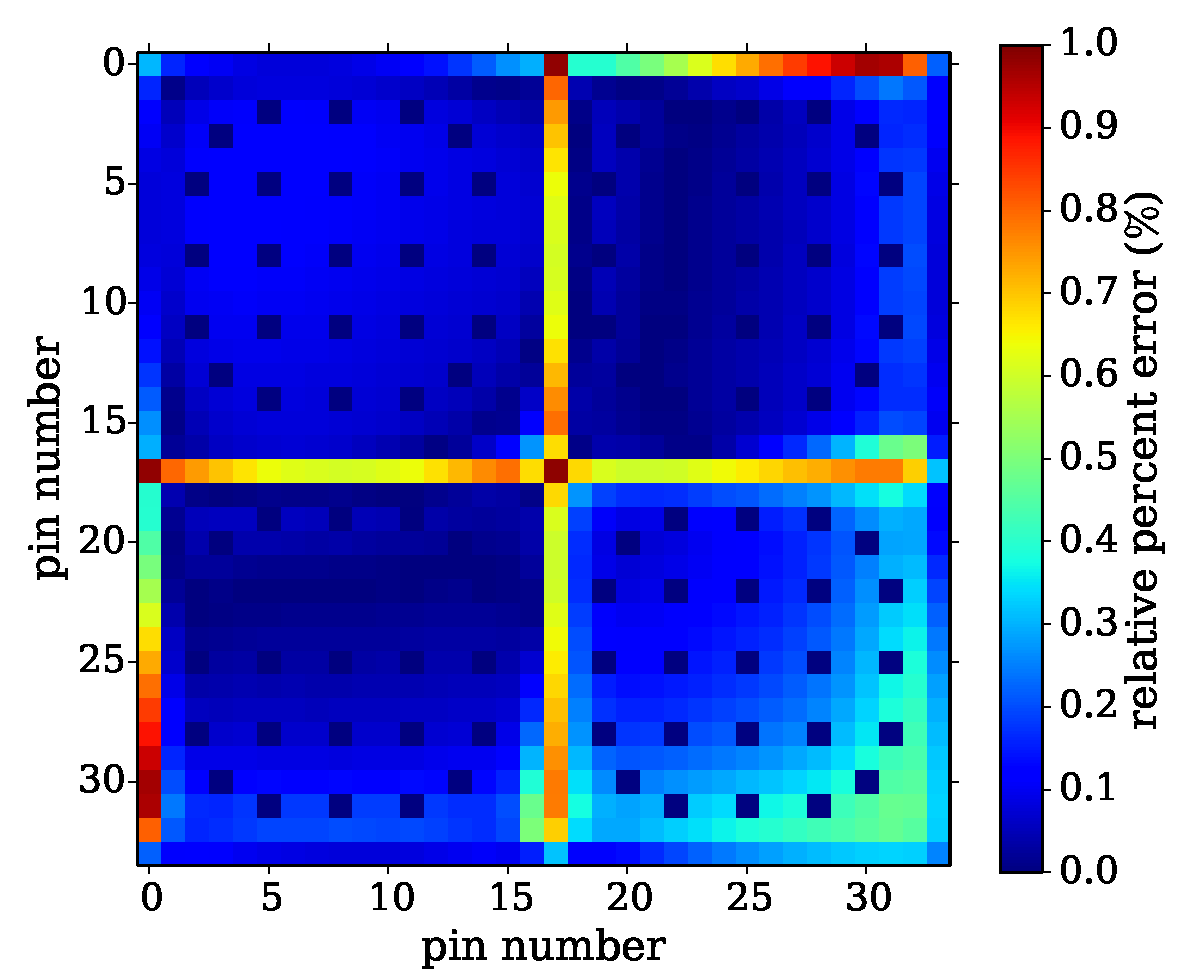
\includegraphics[trim=.1cm .25cm 2.0cm .4cm clip=true, 
    totalheight=0.4\textheight]{Figures/c/c5g7/rf_plots/%
                          phi/serklt8_error}
    \caption{Error in the pin powers of the best performing KLT case (9th 
order, Reduced Small-Core, snapshots of $\phi$) relative to the SERMENT 
reference solution.  The upper left corner is the center of the core}
    \label{fig:serklt}
\end{figure*}

The error heat map for using snapshots of only the partial currents $J_{up}$ and 
$J_{down}$ is presented in \FIG{fig:serkltpl}.  As shown, on average, the pin 
powers are predicted well for the majority of the pins with the exception of 
the center of the core.  The partial current appears to lead to better 
predictions of the pin powers in the 2-D model.

\begin{figure*}[tb]
    \centering
    \includegraphics[trim=.1cm .25cm 2.0cm .4cm clip=true, 
    totalheight=0.4\textheight]{Figures/s/c5g7/rf_plots/%
                          partial/partial_serklt8_error}
    \caption{Error in the pin powers of the best performing KLT case (9th 
order, Reduced Small-Core, snapshots of $J_{up}$ and $J_{down}$) 
relative to the 
SERMENT reference solution.  The upper left corner is the center of the 
core}
    \label{fig:serkltpl}
\end{figure*}

Finally, the error of the best performing KLT case from using $J_{up}$ and $J_{down}$ snapshots 
and $\phi$ snapshots (9th order, Reduced Small-Core) is presented in 
\FIG{fig:serkltpartial}.  The maximum error for the case of including the 
partial current is reduced from the case of only using snapshots of $\phi$, and the location of the 
maximum error has moved to the center of the core model.

\begin{figure*}[tb]
    \centering
    \includegraphics[trim=.1cm .25cm 2.0cm .4cm clip=true, 
    totalheight=0.4\textheight]{Figures/c/c5g7/rf_plots/%
                          partial/partial_serklt8_error}
    \caption{Error in the pin powers of the best performing KLT case (9th 
order, Reduced Small-Core, snapshots of $\phi$, $J_{up}$, and $J_{down}$) relative to the 
SERMENT reference solution.  The upper left corner is the center of the 
core}
    \label{fig:serkltpartial}
\end{figure*}

\section{Conclusion}

The KLT can be effective as compared to the results of mDLP for 2-D models.  In 
general it seems that more degrees of freedom are required in general for the 
C5G7 test problem as compared to the 1-D test problems, but that is expected 
due to the increased difficulty of modeling 2-D problems.  

In general, it seems that the size of the snapshot model is not a strong 
predictor of the success of a basis set.  The Combined-Pins model performs 
surprisingly well despite the model simplicity, and in some cases is the best 
performing in terms of the smallest maximum error at order 9.

The largest errors typically occur at material and assembly junctions, which is 
expected.  The C5G7 benchmark was designed with difficult to capture junctions, 
to increase the difficulty of the benchmark.  It is interesting that the 
including the partial current snapshots moves the largest relative error to the 
center of the core instead of the material junctions.  

Similar the the 1-D results, the best performing basis functions are attained 
on average by including all available snapshots into basis generation.  However 
spatially averaging the snapshots does not appear to have a strong effect on 
the success of the basis set.  This is also expected because the snapshots 
provided by neighboring spatial cells are expected to be exceedingly similar.